
\begin{frameb}{w}{Images/HubbleXDF.png}
	\frametitle{The Big Bang}
	\framesubtitle{Galactic Redshift}
\end{frameb}

\begin{frame}
	\frametitle{The Big Bang}
	\framesubtitle{Galactic Redshift}

	As observed by Edwin Hubble in 1929,
	it appears that:

	\begin{enumerate}
		\pause\item All Galaxies are moving away from us
		\pause\item The Further away they are, the faster they are moving away
		\pause\item If we were to go to another galaxy, we would see exactly the same thing
	\end{enumerate}

\end{frame}


\begin{frameb}{h}{Images/accel_expanding_univ_still_4_300dpi.jpg}
\end{frameb}             
\begin{frameb}{h}{Images/accel_expanding_univ_still_6_300dpi.jpg}
\end{frameb}             
\begin{frameb}{h}{Images/accel_expanding_univ_still_8_300dpi.jpg}
\end{frameb}



\begin{frame}
	\frametitle{The Big Bang}
	\framesubtitle{A stretching universe:}
	\centerline{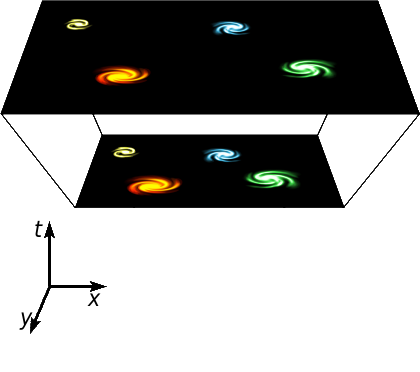
\includegraphics[height=0.8\textheight]{Images/Universe_expansion1.png}}
\end{frame}
\begin{frame}
	\frametitle{The Big Bang}
	\framesubtitle{A stretching universe:}
	\centerline{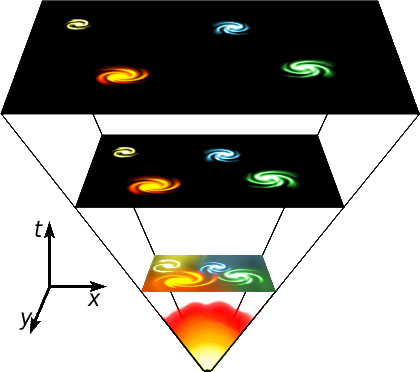
\includegraphics[height=0.8\textheight]{Images/Universe_expansion.png}}
\end{frame}


\begin{frame}
	\frametitle{The Big Bang}
	\framesubtitle{Common Misconceptions}
	The Big Bang does {\em NOT} look like this:
	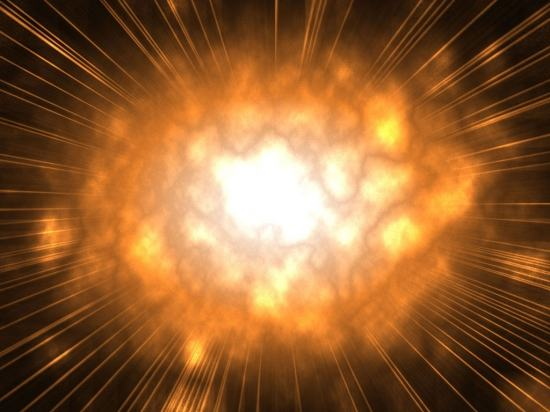
\includegraphics[width=\textwidth]{Images/bigbangnot.jpg}
	
\end{frame}

\begin{frame}
	\frametitle{The Big Bang}
	\framesubtitle{Common Misconceptions}

	\begin{itemize}
		\item Despite the name, the Big Bang is not an explosion.
		\pause\item The Universe is not necessarily expanding into anything.
		\pause\item The big bang didn't begin at a particular point
	\end{itemize}
	
\end{frame}

